\section{Introduction}

This is a sample!  It does not have a lot of fancy stuff in it, but if
you want to see a more complex sample, look at the original ACM
templates.

To fill up enough text to fill up 3 pages, we've included the CCS Call
for Papers three times.  It is always a good idea to include some
gratuitious citations to recent CCS papers~\cite{medvinsky1993netcash,
  bellare1993random, anderson1993cryptosystems, blaze1993cryptographic}.

And here is a plot (\figref{plot-sample}) for the heck of it.

\begin{figure}[h]
\centering
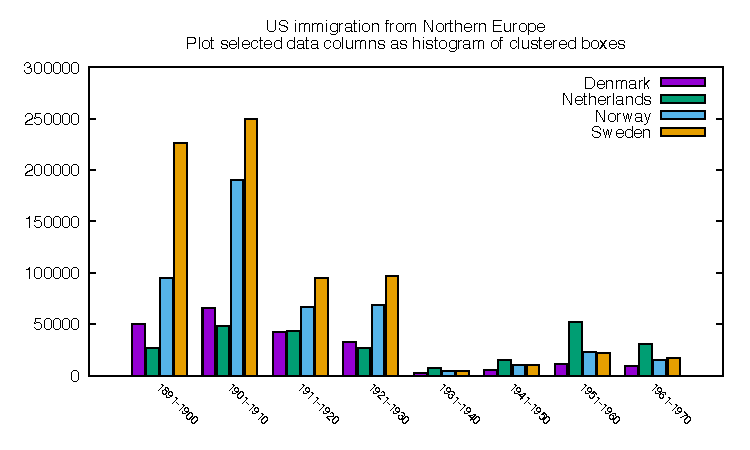
\includegraphics[width=\columnwidth]{plots/plot-sample}
\caption{When America was great.}
\label{fig:plot-sample}
\end{figure}

\section{Call for Papers}

The conference seeks submissions presenting novel research results in
all aspects of computer and communications security and privacy,
including both practical and theoretical contributions.

\subsection{Paper Submission Information}

Submissions must be received at \url{https://ccs17.hotcrp.com/} by the
strict deadline of {\bf 19 May 2017 at 8:59 PM PDT (UTC-7)}.
Submitted papers must not substantially overlap with papers that have
been published or that are simultaneously submitted to a journal,
conference, or workshop. Submissions must be anonymized and avoid
obvious self-references.

CCS has traditionally required that authors submitting papers
guarantee that an author will be able to present their paper at the
conference. We recognize, however, that the current travel
restrictions and screening processes may make it impossible or
uncomfortable for some authors to travel to the conference. The venue
for CCS 2017 was selected several years ago, and we do not wish to
exclude any potential authors who may have difficulty traveling due to
recent changes in US immigration practices.  CCS welcomes submissions
by authors of all nationalities, and will make allowances for
presenting papers electronically or with non-author presenters in
cases where paper authors are unable to travel to the United States.

Submissions will be evaluated based on their scientific merit,
novelty, importance, presentation quality, and relevance to computer
and communications security and privacy.  If a paper includes work
that raises ethical concerns it is up to the authors to convince the
reviewers that appropriate practices were followed to minimize
possible harm and that any harm caused by the work is greatly
outweighed by its benefits. The review process will be carried out in
two phases and authors will have an opportunity to provide a
length-limited response to the first-phase reviews.

\subsection{Paper Format}

Submissions must be single PDF files containing at most 12 pages in
the required new ACM format (see
\url{https://www.sigsac.org/ccs2017/format} for details and templates,
which you have presumably found if you are reading this!) of body
content, with any number of additional pages for the bibliography,
well-marked appendices, and any desired supplementary material.  When
relevant, submitters may include reviews from past submissions and
responses to them in the supplementary material.

Reviewers are not required to consider the appendices or supplementary
material, however, so submissions need to be intelligible and
convincing without them.  Submissions not meeting these guidelines, or
playing games to work around page limits, will be rejected by the PC
chairs without review.  In particular, papers should not use squeezing
tricks to adjust the (already very dense) ACM paper format, and moving
discussion of key related work or important definitions to appendices
may be grounds for rejection.

\subsection{Practice Talks}

Following the lead of USENIX Enigma, we want to improve the quality of
the conference and provide a better experience for both presenters and
attendees by holding practice sessions before the conference (see
\url{https://www.sigsac.org/ccs2017/practicefaq}). Presenting authors
of accepted papers are expected to participate in an on-line practice
session approximately three weeks before the conference.

\subsection{Conflicts of Interest}

The conference requires cooperation from both authors and program
committee members to ensure a process that is both fair in practice
and perceived to be fair by everyone. When submitting a paper, authors
are required to identify members of the program committee who may not
be able to provide an unbiased review.  This includes people with
strong personal or professional relationships such as advisor/advisee,
members of the same organization, and close collaborators (for
example, recent or repeated co-authors). In general, this means anyone
who a reasonable person with all the relevant information would
question as an impartial reviewer. The program co-chairs reserve the
right to request a more specific description of a conflict-of-interest
declaration from authors.

Program committee members who have a conflict of interest with a
paper, including program co-chairs, will be excluded from evaluation
and discussion of the paper, but because submissions are anonymous to
reviewers it is important for submitting authors to identify these
conflicts. In the case of a program co-chair, the other co-chairs who
do not have conflicts will be responsible for managing that paper.
Program co-chairs are not permitted to be involved as co-authors in
any submissions.



\section{Call for Papers}

The conference seeks submissions presenting novel research results in
all aspects of computer and communications security and privacy,
including both practical and theoretical contributions.

\subsection{Paper Submission Information}

Submissions must be received at \url{https://ccs17.hotcrp.com/} by the
strict deadline of {\bf 19 May 2017 at 8:59 PM PDT (UTC-7)}.
Submitted papers must not substantially overlap with papers that have
been published or that are simultaneously submitted to a journal,
conference, or workshop. Submissions must be anonymized and avoid
obvious self-references.

CCS has traditionally required that authors submitting papers
guarantee that an author will be able to present their paper at the
conference. We recognize, however, that the current travel
restrictions and screening processes may make it impossible or
uncomfortable for some authors to travel to the conference. The venue
for CCS 2017 was selected several years ago, and we do not wish to
exclude any potential authors who may have difficulty traveling due to
recent changes in US immigration practices.  CCS welcomes submissions
by authors of all nationalities, and will make allowances for
presenting papers electronically or with non-author presenters in
cases where paper authors are unable to travel to the United States.

Submissions will be evaluated based on their scientific merit,
novelty, importance, presentation quality, and relevance to computer
and communications security and privacy.  If a paper includes work
that raises ethical concerns it is up to the authors to convince the
reviewers that appropriate practices were followed to minimize
possible harm and that any harm caused by the work is greatly
outweighed by its benefits. The review process will be carried out in
two phases and authors will have an opportunity to provide a
length-limited response to the first-phase reviews.

\subsection{Paper Format}

Submissions must be single PDF files containing at most 12 pages in
the required new ACM format (see
\url{https://www.sigsac.org/ccs2017/format} for details and templates,
which you have presumably found if you are reading this!) of body
content, with any number of additional pages for the bibliography,
well-marked appendices, and any desired supplementary material.  When
relevant, submitters may include reviews from past submissions and
responses to them in the supplementary material.

Reviewers are not required to consider the appendices or supplementary
material, however, so submissions need to be intelligible and
convincing without them.  Submissions not meeting these guidelines, or
playing games to work around page limits, will be rejected by the PC
chairs without review.  In particular, papers should not use squeezing
tricks to adjust the (already very dense) ACM paper format, and moving
discussion of key related work or important definitions to appendices
may be grounds for rejection.

\subsection{Practice Talks}

Following the lead of USENIX Enigma, we want to improve the quality of
the conference and provide a better experience for both presenters and
attendees by holding practice sessions before the conference (see
\url{https://www.sigsac.org/ccs2017/practicefaq}). Presenting authors
of accepted papers are expected to participate in an on-line practice
session approximately three weeks before the conference.

\subsection{Conflicts of Interest}

The conference requires cooperation from both authors and program
committee members to ensure a process that is both fair in practice
and perceived to be fair by everyone. When submitting a paper, authors
are required to identify members of the program committee who may not
be able to provide an unbiased review.  This includes people with
strong personal or professional relationships such as advisor/advisee,
members of the same organization, and close collaborators (for
example, recent or repeated co-authors). In general, this means anyone
who a reasonable person with all the relevant information would
question as an impartial reviewer. The program co-chairs reserve the
right to request a more specific description of a conflict-of-interest
declaration from authors.

Program committee members who have a conflict of interest with a
paper, including program co-chairs, will be excluded from evaluation
and discussion of the paper, but because submissions are anonymous to
reviewers it is important for submitting authors to identify these
conflicts. In the case of a program co-chair, the other co-chairs who
do not have conflicts will be responsible for managing that paper.
Program co-chairs are not permitted to be involved as co-authors in
any submissions.



\section{Call for Papers}

The conference seeks submissions presenting novel research results in
all aspects of computer and communications security and privacy,
including both practical and theoretical contributions.

\subsection{Paper Submission Information}

Submissions must be received at \url{https://ccs17.hotcrp.com/} by the
strict deadline of {\bf 19 May 2017 at 8:59 PM PDT (UTC-7)}.
Submitted papers must not substantially overlap with papers that have
been published or that are simultaneously submitted to a journal,
conference, or workshop. Submissions must be anonymized and avoid
obvious self-references.

CCS has traditionally required that authors submitting papers
guarantee that an author will be able to present their paper at the
conference. We recognize, however, that the current travel
restrictions and screening processes may make it impossible or
uncomfortable for some authors to travel to the conference. The venue
for CCS 2017 was selected several years ago, and we do not wish to
exclude any potential authors who may have difficulty traveling due to
recent changes in US immigration practices.  CCS welcomes submissions
by authors of all nationalities, and will make allowances for
presenting papers electronically or with non-author presenters in
cases where paper authors are unable to travel to the United States.

Submissions will be evaluated based on their scientific merit,
novelty, importance, presentation quality, and relevance to computer
and communications security and privacy.  If a paper includes work
that raises ethical concerns it is up to the authors to convince the
reviewers that appropriate practices were followed to minimize
possible harm and that any harm caused by the work is greatly
outweighed by its benefits. The review process will be carried out in
two phases and authors will have an opportunity to provide a
length-limited response to the first-phase reviews.

\subsection{Paper Format}

Submissions must be single PDF files containing at most 12 pages in
the required new ACM format (see
\url{https://www.sigsac.org/ccs2017/format} for details and templates,
which you have presumably found if you are reading this!) of body
content, with any number of additional pages for the bibliography,
well-marked appendices, and any desired supplementary material.  When
relevant, submitters may include reviews from past submissions and
responses to them in the supplementary material.

Reviewers are not required to consider the appendices or supplementary
material, however, so submissions need to be intelligible and
convincing without them.  Submissions not meeting these guidelines, or
playing games to work around page limits, will be rejected by the PC
chairs without review.  In particular, papers should not use squeezing
tricks to adjust the (already very dense) ACM paper format, and moving
discussion of key related work or important definitions to appendices
may be grounds for rejection.

\subsection{Practice Talks}

Following the lead of USENIX Enigma, we want to improve the quality of
the conference and provide a better experience for both presenters and
attendees by holding practice sessions before the conference (see
\url{https://www.sigsac.org/ccs2017/practicefaq}). Presenting authors
of accepted papers are expected to participate in an on-line practice
session approximately three weeks before the conference.

\subsection{Conflicts of Interest}

The conference requires cooperation from both authors and program
committee members to ensure a process that is both fair in practice
and perceived to be fair by everyone. When submitting a paper, authors
are required to identify members of the program committee who may not
be able to provide an unbiased review.  This includes people with
strong personal or professional relationships such as advisor/advisee,
members of the same organization, and close collaborators (for
example, recent or repeated co-authors). In general, this means anyone
who a reasonable person with all the relevant information would
question as an impartial reviewer. The program co-chairs reserve the
right to request a more specific description of a conflict-of-interest
declaration from authors.

Program committee members who have a conflict of interest with a
paper, including program co-chairs, will be excluded from evaluation
and discussion of the paper, but because submissions are anonymous to
reviewers it is important for submitting authors to identify these
conflicts. In the case of a program co-chair, the other co-chairs who
do not have conflicts will be responsible for managing that paper.
Program co-chairs are not permitted to be involved as co-authors in
any submissions.




\section{Conclusions}

In conclusion, it is rarely a good idea to include the same section three times in a paper, or to have a conclusion that does not conclude.
%
But never mind that. We have the president's authorization (see \figref{president-sig}) to go on. Let's make this paper great again!

\begin{figure}[h]
\centering

\includegraphics[width=.75\columnwidth]{figs/fig-sample}
\caption{The President's signature of approval.}
\label{fig:president-sig}
\end{figure}

\appendix

\section{Location}

Note that in the new ACM style, the Appendices come before the References.

\section{Call for Papers}

The conference seeks submissions presenting novel research results in
all aspects of computer and communications security and privacy,
including both practical and theoretical contributions.

\subsection{Paper Submission Information}

Submissions must be received at \url{https://ccs17.hotcrp.com/} by the
strict deadline of {\bf 19 May 2017 at 8:59 PM PDT (UTC-7)}.
Submitted papers must not substantially overlap with papers that have
been published or that are simultaneously submitted to a journal,
conference, or workshop. Submissions must be anonymized and avoid
obvious self-references.

CCS has traditionally required that authors submitting papers
guarantee that an author will be able to present their paper at the
conference. We recognize, however, that the current travel
restrictions and screening processes may make it impossible or
uncomfortable for some authors to travel to the conference. The venue
for CCS 2017 was selected several years ago, and we do not wish to
exclude any potential authors who may have difficulty traveling due to
recent changes in US immigration practices.  CCS welcomes submissions
by authors of all nationalities, and will make allowances for
presenting papers electronically or with non-author presenters in
cases where paper authors are unable to travel to the United States.

Submissions will be evaluated based on their scientific merit,
novelty, importance, presentation quality, and relevance to computer
and communications security and privacy.  If a paper includes work
that raises ethical concerns it is up to the authors to convince the
reviewers that appropriate practices were followed to minimize
possible harm and that any harm caused by the work is greatly
outweighed by its benefits. The review process will be carried out in
two phases and authors will have an opportunity to provide a
length-limited response to the first-phase reviews.

\subsection{Paper Format}

Submissions must be single PDF files containing at most 12 pages in
the required new ACM format (see
\url{https://www.sigsac.org/ccs2017/format} for details and templates,
which you have presumably found if you are reading this!) of body
content, with any number of additional pages for the bibliography,
well-marked appendices, and any desired supplementary material.  When
relevant, submitters may include reviews from past submissions and
responses to them in the supplementary material.

Reviewers are not required to consider the appendices or supplementary
material, however, so submissions need to be intelligible and
convincing without them.  Submissions not meeting these guidelines, or
playing games to work around page limits, will be rejected by the PC
chairs without review.  In particular, papers should not use squeezing
tricks to adjust the (already very dense) ACM paper format, and moving
discussion of key related work or important definitions to appendices
may be grounds for rejection.

\subsection{Practice Talks}

Following the lead of USENIX Enigma, we want to improve the quality of
the conference and provide a better experience for both presenters and
attendees by holding practice sessions before the conference (see
\url{https://www.sigsac.org/ccs2017/practicefaq}). Presenting authors
of accepted papers are expected to participate in an on-line practice
session approximately three weeks before the conference.

\subsection{Conflicts of Interest}

The conference requires cooperation from both authors and program
committee members to ensure a process that is both fair in practice
and perceived to be fair by everyone. When submitting a paper, authors
are required to identify members of the program committee who may not
be able to provide an unbiased review.  This includes people with
strong personal or professional relationships such as advisor/advisee,
members of the same organization, and close collaborators (for
example, recent or repeated co-authors). In general, this means anyone
who a reasonable person with all the relevant information would
question as an impartial reviewer. The program co-chairs reserve the
right to request a more specific description of a conflict-of-interest
declaration from authors.

Program committee members who have a conflict of interest with a
paper, including program co-chairs, will be excluded from evaluation
and discussion of the paper, but because submissions are anonymous to
reviewers it is important for submitting authors to identify these
conflicts. In the case of a program co-chair, the other co-chairs who
do not have conflicts will be responsible for managing that paper.
Program co-chairs are not permitted to be involved as co-authors in
any submissions.




\begin{acks}
% TODO: For the submission, don't include acknowledgments since they would most likely deanonymize you.
\end{acks}
